\chapter{Process Simulation}

Process simulation is a versatile quantitative analysis method that can be used for both as-is and what-if analyses. It involves running a large number of process instances, navigating through the state space, gathering performance data such as cost, time, and resource usage, and then calculating statistics from the collected data. This method is particularly useful for validation and performance analysis, although it cannot be used to prove the correctness of a process. At best, simulation can reveal flaws by chance during a run. It is the most widely used model-based technique to improve process executions.

\section{Advantages and Limitations of Simulation}

Simulation offers several advantages. It reduces the risks and costs associated with conducting real-world experiments. By testing the performance at the level of a model rather than on the spot, such as in a manufacturing line or healthcare setting, simulation can be a safer and more cost-effective alternative. Real-world experiments can often be too costly or dangerous to perform, such as experimenting on hospital patients.

However, simulation also has its limitations. It relies heavily on the realism of the process model. Encoding every aspect of a process can be non-trivial, leading to low precision. If the simulation model is not realistic and accurate, the optimization results will be theoretical and not reflective of reality.

\section{Steps in Process Simulation}

To conduct a process simulation, follow these steps:

\subsection{Model the Process}

The first step is to model the process using Business Process Model and Notation (BPMN). 
\begin{figure}[h!]
    \centering
    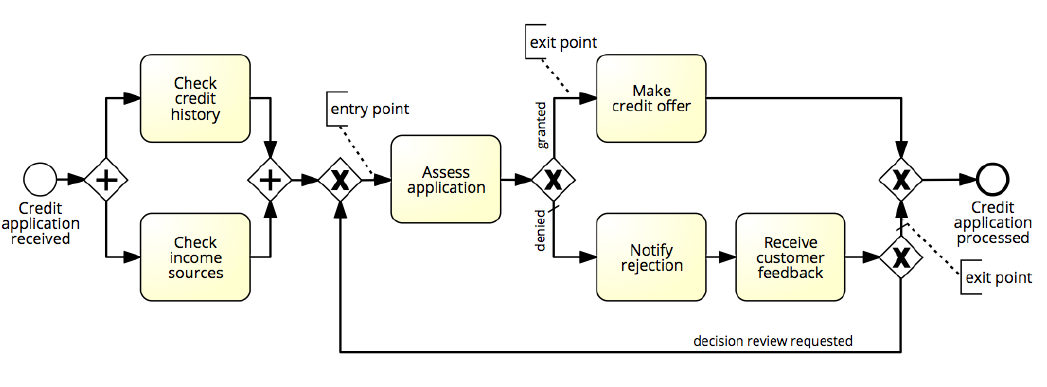
\includegraphics[width=0.75\linewidth]{capitolo 10/1.png}
\end{figure}
This involves defining a simulation scenario, which includes several key components:

Processing times of activities can be fixed values or follow a probability distribution. The choice of distribution depends on the nature of the activity. For example, a fixed value can be used for tasks with little variation in processing time, such as those performed by software applications. A normal distribution is suitable for simple and repetitive activities with minimal human judgment, like checking the completeness of an application. An exponential distribution is appropriate for complex activities involving analysis or decisions, such as assessing an application.
\begin{figure}[h!]
    \centering
    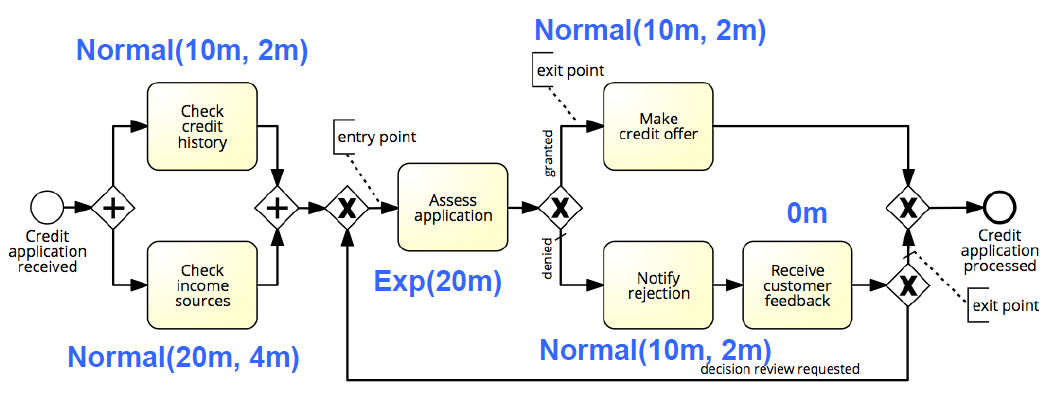
\includegraphics[width=0.75\linewidth]{capitolo 10/2.png}
\end{figure}
\begin{figure}[h!]
    \centering
    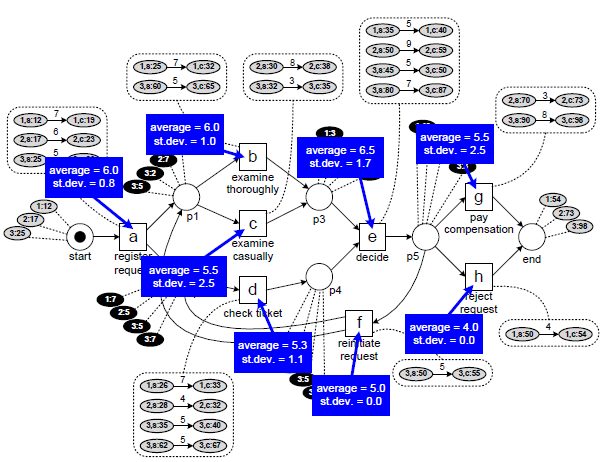
\includegraphics[width=0.75\linewidth]{capitolo 10/3.png}
\end{figure}

Branching probabilities are obtained by replaying the event-log traces onto the model. If the traces are not replayable, it may be necessary to create alignments.
\begin{figure}[h!]
    \centering
    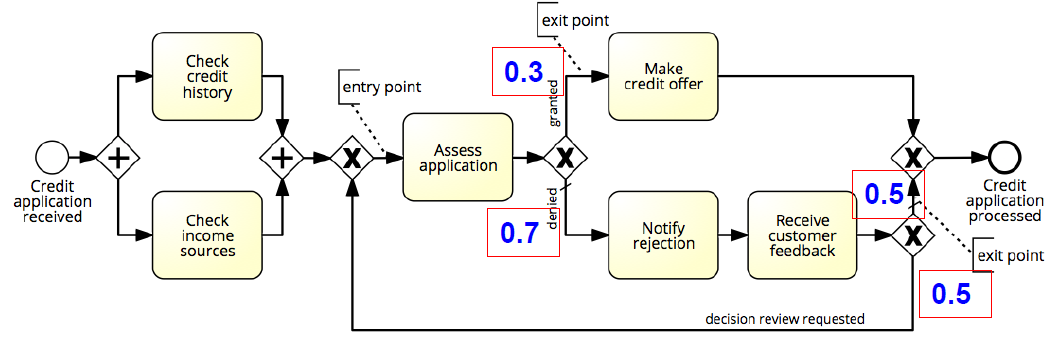
\includegraphics[width=0.75\linewidth]{capitolo 10/4.png}
\end{figure}
The arrival rate of process instances typically follows an exponential distribution with a given mean inter-arrival time. The arrival calendar, such as Monday to Friday from 9 am to 5 pm, or 24/7, should also be defined.

Resource pools should be defined with their name, size, cost per time unit, and availability (working calendar). In some tools, it is possible to define cost and calendar per resource rather than for the entire resource pool. A resource pool is a set of resources or roles that can perform a given activity. These pools can be constructed from event logs using algorithms to discover roles.
\begin{figure}[h!]
    \centering
    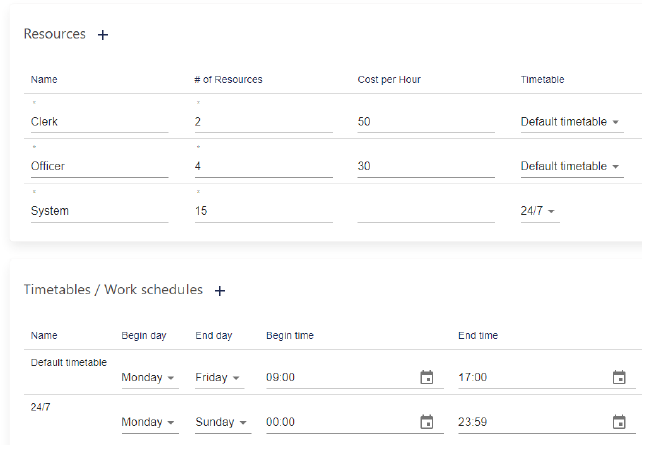
\includegraphics[width=0.75\linewidth]{capitolo 10/5.png}
\end{figure}
\begin{figure}[h!]
    \centering
    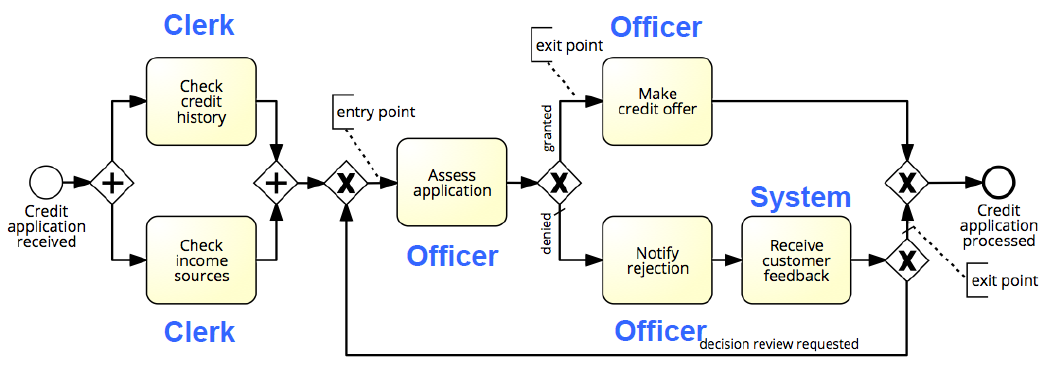
\includegraphics[width=0.75\linewidth]{capitolo 10/6.png}
\end{figure}

\subsection{Run the Simulation and Analyze Outputs}

After defining the simulation scenario, the next step is to run the simulation and analyze the outputs. This involves gathering performance data such as cost, time, and resource usage, and then calculating statistics from the collected data. It is important to analyze the simulation outputs carefully, as they provide insights into the behavior of the process under different scenarios.
\begin{figure}[h!]
    \centering
    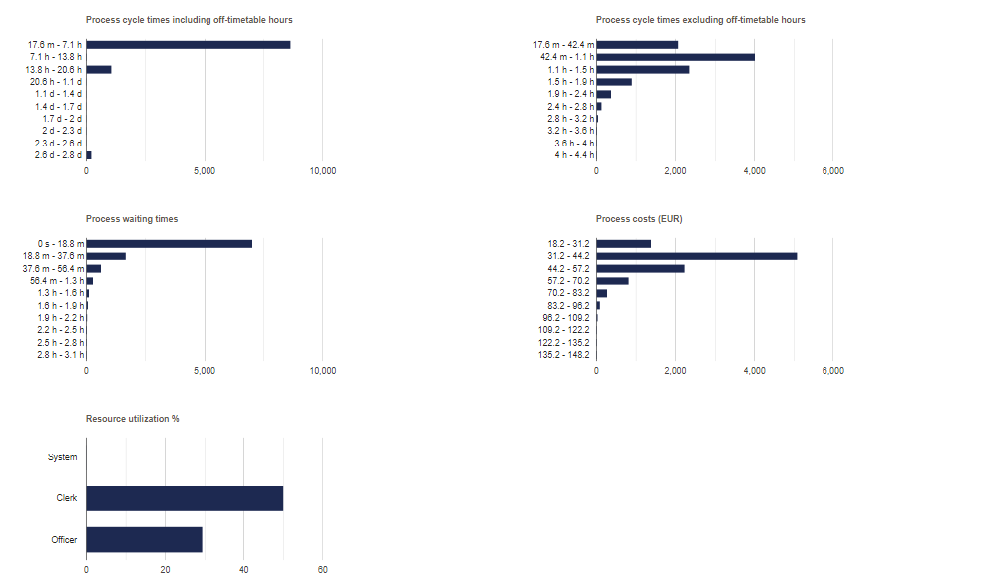
\includegraphics[width=1\linewidth]{capitolo 10/7.png}
\end{figure}

\begin{figure}[h!]
    \centering
    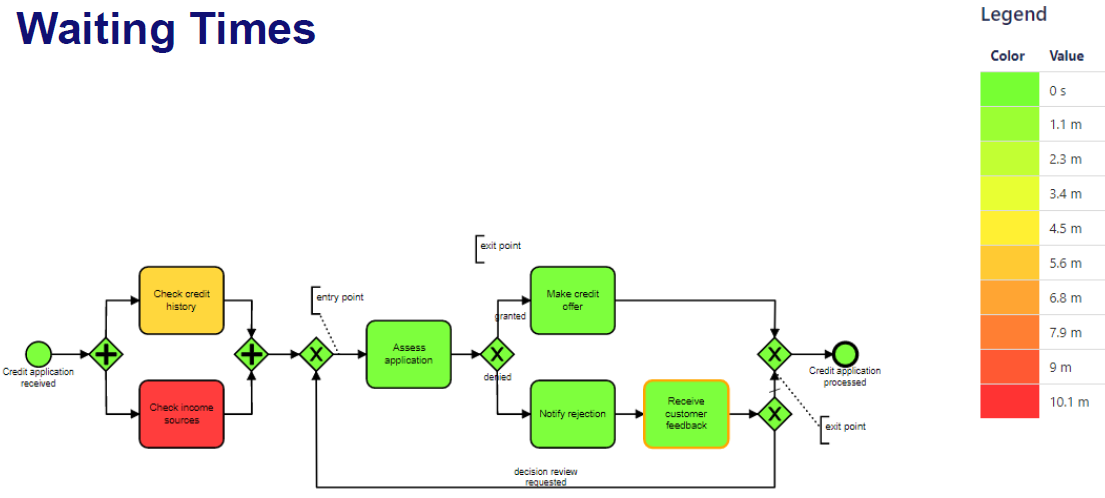
\includegraphics[width=0.75\linewidth]{capitolo 10/8.png}
\end{figure}

\newpage
\subsection{Repeat for Alternative Scenarios}

What-if analysis is a data-intensive simulation that involves inspecting the behavior of a complex system, such as a business process, under given hypotheses called scenarios. The goal is to measure how changes in a set of independent simulation variables impact dependent variables. Formulating a scenario enables building a hypothetical world that analysts can inspect and navigate for improvement.

\section{Pitfalls of Simulation}

While simulation is a powerful tool, it is not without its pitfalls. Stochasticity, data quality, and simplifying assumptions can all affect the reliability of simulation results.

\subsection{Stochasticity}

A single run does not provide information about the reliability of results. Therefore, multiple runs are necessary. If the runs are assumed to be mutually independent, one can calculate a confidence interval. For example, the cycle time is with 95\% confidence within the interval of [5,6] days. It is important to estimate the reliability of the estimates. The size of the confidence interval depends on the confidence level, the length, and the number of simulation runs.

\subsection{Warm-up and Cool-down Periods}

At the beginning of simulations, resources are 100\% free and queues at activities are empty, making the waiting and cycle times of the first traces not trustworthy. Therefore, simulation statistics should not be collected for the first X\% of the traces. Similarly, towards the end of simulations, when every trace of simulation is started, the activity queues become emptier and emptier, making the waiting and cycle times of the last traces not trustworthy. Therefore, simulation statistics should not be collected for the last Y\% of the traces.
\begin{figure}[h!]
    \centering
    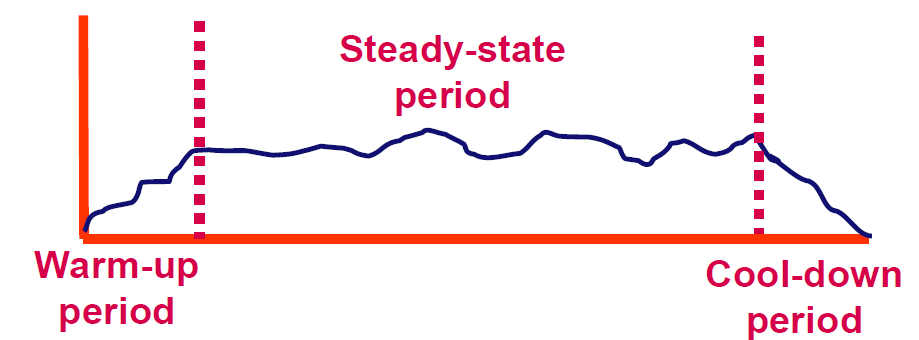
\includegraphics[width=0.75\linewidth]{capitolo 10/9.png}
\end{figure}
\subsection{Data Quality and Simplifying Assumptions}

Simulation results are only as trustworthy as the input data. Therefore, it is important to rely as little as possible on guesstimates and use actual observations where possible. Derive simulation scenario parameters from actual observations, such as applying process mining, and use statistical tools to check the fit of probability distributions. Simulate the as-is scenario and cross-check results against actual observations.

The closed-world assumption is typically used, limiting the input data to every aspect considered. In business process simulation, this means every event is stored in the system. However, some activities and happenings outside the system may not be stored, such as private phone calls, coffee breaks, or colleagues asking questions. To address this, model some invisible waiting-time activities and set their duration according to the waiting times.
